\section{Radiography invention: digital radiography}
A quick Google search on ``radiography breakthrough" suffices to show that
digital radiography is the most significant invention for basic radiography in
recent decades. As mentioned earlier in \autoref{ssec:recentradio}, digital
radiographs are much easier to store, copy, post-process share compared to their
analogue siblings. Additionally, unlike radiographic film there is no potential
for over- or underexposure. Instead, the output can be rescaled as needed during
post-processing. Some techniques also allow for a reduced exposure of the
patient, minimizing the risk. The ubiquity of digital scanners these days prove
that the advantages outclass the disadvantages. However, these disadvantages do
exist. Analogue images have a very high inherent resolution, and by examining
them on a lightbox the contrast is unmatched by any kind of computer screen. In
addition, because analogue systems do not use digital electronics, there is no
electronic noise. Digital radiographs do not have necessarily to outclass their
analogue counterparts on these fronts, but they have to achieve a minimum level
to make sure their diagnostic value is not impaired.

\subsection{Defining the technology}
What makes radiography analogue or digital depends on kind of detector used.
Other parts of the scanner such as the X-ray source do not have to be altered
to make the transition. Furthermore, it is not one specific technology that
makes this transition possible. Various components are needed, and for each
of them there are some alternatives as well. On top of that, evolution in other
fields such as digital electronics and computer machinery had to be advanced
enough to take full advantage of the possibilities. 

\begin{figure}[ht]
\begin{center}
  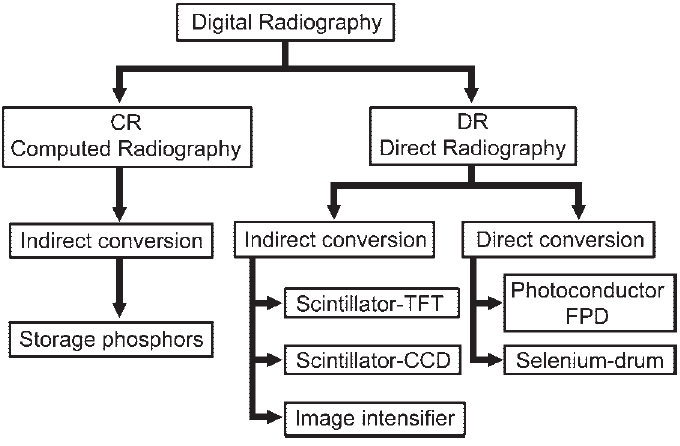
\includegraphics[width=\linewidth]{img/radiohierarchie.png}
  \caption{A systematic overview of various types of digital detectors. CCD =
  chargecoupled device, FPD = flat-panel detector, TFT = thin-film transistor.
  \cite{digitalradio}}
  \label{fig:radiohierarchie}
\end{center}
\end{figure} 

We first discuss the various types in greater detail using
\autoref{fig:radiohierarchie}. The first incarnation of digital radiography -
called computed radiography (CR) - used storage phosphor to temporarily store
the image information, and lasers to read out the values pixel by pixel at a later
stage \cite{digitalradio}. Unfortunately, the physical properties of storage
phosphors severely limited the resolution of the resulting image, reducing their
diagnostic value. The technology underwent many iterations, as shown in
\autoref{tbl:radiotime}.

\begin{table}[ht]
\begin{tabular}{l l}
\hline
Year & Development\\
\hline
1980 & Computed radiography (CR), storage phosphors\\
1987 & Amorphous selenium�based image plates\\
1990 & Charge-coupled device (CCD) slot-scan direct radiography (DR)\\
1994 & Selenium drum DR\\
1995 & Amorphous silicon�cesium iodide (scintillator) flat-panel detector\\
1995 & Selenium-based flat-panel detector\\
1997 & Gadolinium-based (scintillator) flat-panel detector\\
2001 & Gadolinium-based (scintillator) portable flat-panel detector\\
2001 & Dynamic flat-panel detector fluoroscopy�digital subtraction angiography\\
\hline
\end{tabular}
\caption{Timetable of developments in digital radiography \cite{digitalradio}.}
\label{tbl:radiotime}
\end{table}

The alternative to computed radiography is direct radiography (DR). It comes in
two forms, using either direct or indirect conversion. The direct form uses a
photoconductor to convert the incident photons to electrical charges. Typical
semiconductor materials used in photoconductors are amorphous Selenium (a-Se)
and Gadolinium (Gd). In earlier versions the photons were projected onto a
rotating drum and converted to electrical signals using an analog to digital
converter (ADC). Newer versions however use a flat panel detector (FDP) where
the ADC is swapped out for thin-film transistors (TFT, also used in LCD
displays). These TFTs are made of amorphous Silicon (a-Si). Because the used
materials have a very high intrinsic resolution, the final image resolution is
only limited by the kind of detector used.

\begin{figure}[ht]
\begin{center}
  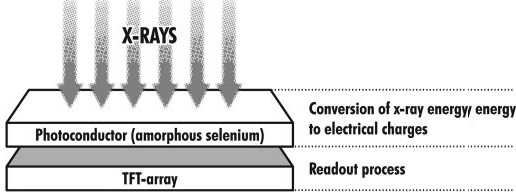
\includegraphics[width=\linewidth]{img/direct_FPD.png}
  \caption{Components of a direct conversion flat panel detector. \cite{digitalradio}}
  \label{fig:directfpd}
\end{center}
\end{figure}

In indirect conversion DR, an extra element is added between the X-rays and the
actual detector. A common example is a scintillator plate that converts X-rays
into visible light. Alternatively, an image intensifier (II) can be used to
amplify the light output. This light can than be captured more easily by a
charge-coupled device (CCD, also used in digital cameras) or a TFT. Because of
the extra step, the point spread function (PSF) increases and the resolution
suffers slightly.

A CCD chip is relatively small so it cannot under normal circumstances record a
whole image at once. Two alternatives are possible. One uses a lens to focus the
rays onto the smaller chip area, but this reduces the image quality. Another
uses a small collimated fan-shaped beam combined with a moving CCD detector.
This system performs comparable to FPDs. One drawback is that this elaborate
setup is not very mobile.

Instead of a CCD, TFTs can also be used in a similar fashion as in direct
conversion DR FPDs. Only this time a scintillator is added. These scintillators
use either Cesium Iodide (CsI) or Gd-based crystals. Contrary to Gd, CsI
crystals can be structured, improving the image quality. The trade-off is their
brittleness, making them less portable. The visible light they emit is then
captured by photo diodes and read out by a TFT array.

\begin{figure}[ht]
\begin{center}
  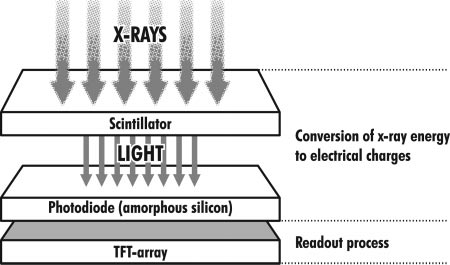
\includegraphics[width=\linewidth]{img/indirect_FPD.png}
  \caption{Components of an indirect conversion flat panel detector. \cite{digitalradio}}
  \label{fig:indirectfpd}
\end{center}
\end{figure}

For the actual assessment, we will focus on both direct and indirect FPDs.

\subsection{Assessing novelty in functionality}
Functionality-wise, we can distinguish between novelty in components and
combinations thereof on the one hand, and novelty in natural effects exploited
on the other hand.

\subsubsection{Novelty in components}
As explained above, digital radiography in general uses many of the same parts
as analogue radiography. Only the detector is fundamentally different. Of course
the real advantage of digitizing radiographs is what you can do with them
afterwards. However, that is out of the scope of this text, and we will
constrain ourselves to the hardware aspects for now.

The next question we ask ourselves is whether these new (combinations) of
components were already used before. The answer is yes. For example CCDs were
invented in 1969 at AT\&T Bell Labs (patents: US3792322,  US3796927) and first
used in digital cameras by 1975 \cite{solidstatesens}. On the other hand, the
combination of a scintillator with CCDs to capture X-rays was not used before. 

In the case of direct FPDs using TFTs, the results are similar. Engineers
experimented with them as early as 1971 for use in display equipment
\cite{lcdhistory}. To this day, they are almost exclusively used in LCD panels
and in digital radiography. In conclusion, they were used before, but mostly in
a field that is not closely related to medical imaging.

\subsubsection{Novelty in natural effects exploited}
Of course the primary natural effect exploited is that of the X-ray passing
through tissue. This has not changed with digital radiography. On the other
hand, the natural effects used in the detector are very distinct from classic
photographic film. Where such films fall under the accomplishments of material
science, modern digital recording equipment are made possible by advances in the
electronic and semiconductor industry. Obviously these natural effects were
exploited numerous times before by other digital equipment, but not equipment
related to medical imaging.

\subsubsection{Scores}
In \autoref{tbl:funcscores1} we give an overview of the scores on the various
topics.

\begin{table}[h]
\centering
\begin{tabular}{l l}
\hline
\multicolumn{2}{|c|}{Novelty in functionality} \\
\hline
A. Novelty of components & B. Novelty in natural effects exploited\\
A1) 4 & B1) 8\\ 
A2) 5 & B2) 5\\ 
\hline
\end{tabular}
\caption{Novelty in functionality scores}
\label{tbl:funcscores1}
\end{table}

\subsection{Assessing novelty in knowledge origins}
Regarding knowledge origins (KOs), we can make a distinction between scientific
and technological origins. To find these KOs, we first provide a list of
problems that had to be solved for digital radiography to become feasible.

The main purpose is to somehow intercept the X-rays and translate their
intensities per pixel into a discrete values that can be processed by a
computer. To do so, they X-rays must first be converted to electrical charges,
which can then be interpreted as bits.

Problem 1: converting the X-ray intensities to bits

Problem 1.1: converting the X-rays to electrical charges

Solution 1.1a: direct conversion: use a photoconducting material (a-Se)

KO1: electromagnetism, semiconductors

Solution 1.1b: indirect conversion: use a scintillator (CsI) and photodiodes (a-Si)

KO2: electromagnetism, material science and semiconductors

Problem 1.2: converting the electrical charges to bits

Solution 1.2: use a TFT array

KO3: digital electronics (mostly transistors)

\subsubsection{Scores}
Electromagnetism falls under scientific origins. The use of electromagnetism
knowledge in medical imaging is certainly nothing special, so it receives low
scores.

The other origins fit better in the technological group. The use of digital
electronics and all related disciplines makes digital radiography what it is.
This warrants a high score, at least for the detector part. However, at
the time of invention the digital electronics industry was booming and
already widely in use in various other fields. In that regard it was only a
matter of time before someone came up with the idea to combine digital
electronics with radiography.

\autoref{tbl:origscores1} shows the scores.

\begin{table}[h]
\centering
\begin{tabular}{l l}
\hline
\multicolumn{2}{|c|}{Novelty in knowledge origins} \\
\hline
A. Novelty of scientific origins & B. Novelty of technological origins\\
A1) 2 & B1) 8\\ 
A2) 2 & B2) 5\\ 
\hline
\end{tabular}
\caption{Novelty in knowledge origins scores}
\label{tbl:origscores1}
\end{table}

\subsection{Assessing technological impact}
The last part of this digital radiography assessments looks into technological
impact. Impact can be split into three parts: performance increase,
technological accumulation and obsoleting previous technologies.

\subsubsection{Performance increase}
The goal of radiography is simply to make clear images that have a high
diagnostic value. To that end, spatial resolution, contrast and noise as
discussed in \ref{sssec:imgquality} are all important. The aim of digital
resolution was not necessarily to do better in this regard, because analogue
images were already very detailed. If the quality is on par, we should consider
ourselves happy.

As explained above, resolution was a problem with computer radiography using
storage phosphors. However, the materials used in flat panel detectors all have
a high inherent spatial resolution. Only the size of the underlying TFT array
limits the final image resolution. Because analogue radiographs are not
expressed in number of pixels, the performance comparison is complicated.
However, tests performed by \cite{review} show that diagnostic value of analogue
and digital images are almost on par as long as the pixels are about 0.1mm in
size.

Contrast on the other hand is a serious problem for digital radiography. The
deep blacks of photographic film combined with the strong light from a lightbox
creates very high contrast. In comparison, radiologists now have to look at
images on their computer screen in a dark room. On the other hand, digital
radiography makes up for this defect by offering the possibility of
post-processing where it is not only possible to zoom in spatially, but also on
a certain intensity interval (i.e., so-called grey-level transformations
\cite{suetens}).

Noise-wise, the electronic circuits introduce additional electronic noise on top
of the electromagnetic noise. Modern electronics can minimize the former noise,
as evident by our crisp digital photographs a big flat screens.

Other advances in performance include: lack of geometric distortion, no veiling
glare, uniform response across the field of view \cite{review}. In addition,
costs are reduces because expensive photographic film is no longer needed, and
time span is reduces because film development happens automatically and almost
instantly.

It is difficult to assign a single score to this component because of the many
issues at play. The image quality did not necessarily improve much, but this was
not the goal. The real performance increase is due to indirect opportunities
opened up by the digital image format. Therefore, in our opinion this still
deserves a fairly high score.

\subsubsection{Technological accumulation}
In this section we estimate the broadness, magnitude and novelty of the impact.

\paragraph{Broadness of impact}
The real breakthrough that made digital radiography possible was the
advent of digital electronics. This breakthrough had a very broad impact on
fields other than its own. Other fields looked directly at digital electronics,
rather than digital radiography, for possible innovations. That is why this
innovation does not score high on broadness of impact. It did however impact
related fields such as CT and PET.

\paragraph{Magnitude of impact}
Although the broadness of impact was not big, and it mostly concentrated on
highly related fields, the magnitude was considerable. In fact, computed
tomography would not even be possible if it were not for the invention of
digital detectors. The same goes (to a lesser extent) for detectors used in
nuclear medicine imaging.

\paragraph{Novelty of impact}
The novelty of impact of digital radiography is very low because other
technologies that never used digital electronics before, got their ideas from
digital electronics in general, not specifically from digital radiography.

\subsubsection{Obsoleting previous technologies}
The last aspect of impact assessment is obsoleting previous technologies, i.e.
analogue radiography. According to \cite{review} and \cite{suetens}, this has
indeed happened. Few radiology departments still stick with analogue systems
because of their lower cost and extreme reliability, but most of the world has
permanently moved on. Not only in radiography, but also in related disciplines
such as CT and PET.

\subsubsection{Scores}
\autoref{tbl:impactscores1} shows the final scores.

\begin{table}[h]
\centering
\begin{tabular}{l l l}
\hline
\multicolumn{3}{|c|}{Technological impact} \\
\hline
A. Performance increase & B. Tech. accumulation & Obsoleting previous tech.\\
A) 8 & B1 a) 3 --- b) 1 & C) 10\\ 
     & B2 a) 8 --- b) 7 & \\
     & B3 a) 1 --- b) 1 & \\
\hline
\end{tabular}
\caption{Technological impact scores}
\label{tbl:impactscores1}
\end{table}